\documentclass[a4paper,11pt]{article}
\usepackage[utf8]{inputenc}
\usepackage[T1]{fontenc}
\usepackage[a4paper,top=1in, bottom=1in, left=1in, right=1in]{geometry}
\usepackage[french,magyar]{babel}
\def\magyarOptions{defaults=prettiest}

\usepackage[none]{hyphenat}
\usepackage{amsfonts,amsmath,amssymb}
\usepackage{fancyhdr}
\usepackage[none]{hyphenat}

\usepackage{hyperref}
\hypersetup{
    colorlinks=true,
    linkcolor=black,
    filecolor=magenta,      
    urlcolor=blue,
}
\usepackage{float}
\usepackage[dvipsnames]{xcolor}
\usepackage[nottoc,notlot,notlof]{tocbibind}
\usepackage{graphicx}
\usepackage{caption}
\usepackage{subfig}
\usepackage{enumitem}
\usepackage{booktabs}
\usepackage[export]{adjustbox}
\usepackage{enumitem}
\setlist[1]{itemsep=-5pt}
\pagestyle{fancy}
\fancyhead{}
%\fancyfoot{}
\renewcommand{\headrulewidth}{0pt}

\usepackage{hyperref}

\usepackage{listings}
 
\urlstyle{same}

%\renewcommand{\baselinestretch}{1.5}

\begin{document}
%\emergencystretch 3em
\sloppy

\begin{titlepage}
\begin{center}
%\vspace{1cm}
\begin{figure}[t!]
	\begin{center}
	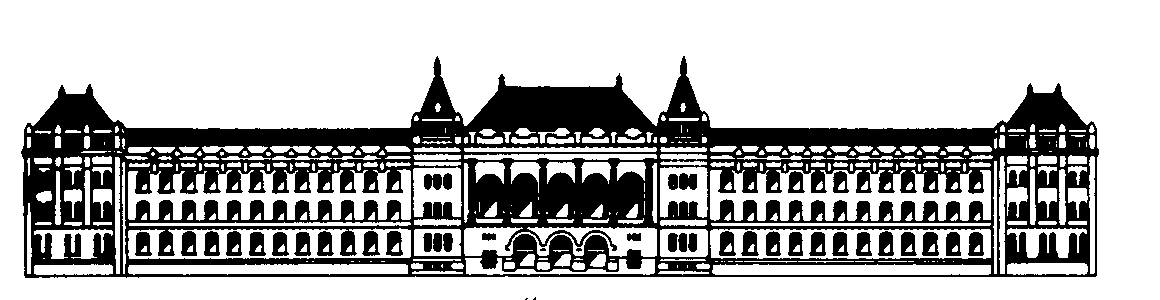
\includegraphics[scale=0.2]{bme.png}
	\label{a:bme}
	\end{center}
\end{figure}
\textbf{{Budapesti Műszaki és Gazdaságtudományi Egyetem}}\\
Villamosmérnöki és Informatikai Kar\\
Méréstechnika és Információs Rendszerek Tanszék\\
\vfill
\huge\textbf{{Logikai tervezés}}\\[3mm]
\Large{Házi feladat}\\[3mm]
\Large\textbf{{Programozható jelgenerátor}}\\
\vfill
\Large{Kardos Bálint, ZI84PX}\\
\Large{Murányi Péter, A74MW9}\\
\Large{Konzulens: Dr. Fehér Béla}\\
\vfill
\today \\

\end{center}
\end{titlepage}

\tableofcontents
\thispagestyle{empty}
\clearpage

\setcounter{page}{1}
\setcounter{tocdepth}{4}
\setcounter{secnumdepth}{4}
\setlength{\parindent}{0em}
\setlength{\parskip}{1em}
\section{Feladat}

%TODO Bálint

\section{Tervezés}

%TODO Bálint
%Blokkdiagramm a DDS belsejéről 
%írd le hogy az egész cuccnak mit kell tartalmaznia

%Rendszerről csináltam
\begin{figure}[h!]
	\begin{center}
		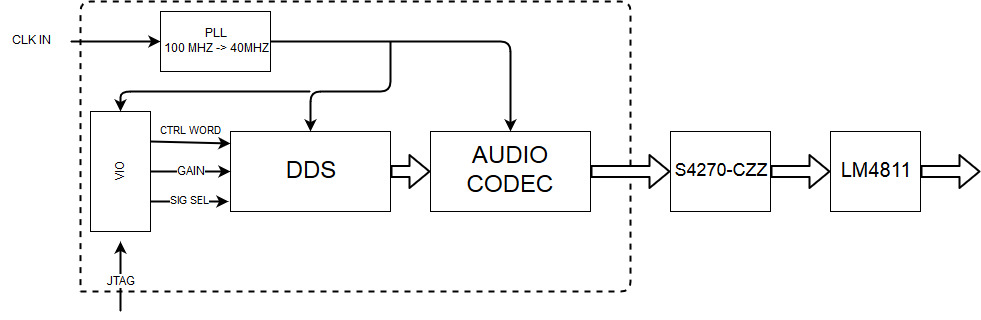
\includegraphics[scale=0.48]{system_block.jpg}	
	\end{center}
	\caption{Rendszer blokkdiagramja}
	\label{a:DDSsystem}
\end{figure}

\section{Megvalósítás}

\subsection{DDS}

A DDS modul tartalmazza a digitális jelet létrehozó hardvert. Az egész modul szinkron a rendszer 40MHz-s jelével, minden egység rendelkezik reset bemenettel, ami valamilyen kezdeti állapotba állítja azt. A modul belső funkciók szerint van szétosztva és megírva. A hullámformák párhuzamosan generálódnak, majd egy multiplexerrel választódik ki a megfelelő kimenet, ami egy szorzóval skálázódik.

Az első rész maga a NCO, ez verilogban nem több mint egy 24 bites regiszter amihez minden felfutó élen hozzáadjuk a vezérlő szavat. Az így kapott jel fogja a bemenetet képezni az összes többi alegységre. A számláló reset jellel nullázható.

A következő rész végzi a szinusz hullám generálását. A szinusz jel létrehozására egy LU-otT (LookUp Table) használunk. Ez a LUT tartalmazza a szinusz értékeit, mivel 24 bites a kimenet, így 24 bites előjeles formában. A LUT 1024 elemből áll, tehát 10 bites a címbemenete, és mivel minden extra bit felbontás 6 dB-t jelent a dinamika tartományban, így csak a szinusz egy negyede van eltárolva. Ahhoz hogy ebből az egy negyedből egy teljes szinuszt kapjunk, mind a LUT ki és bemenetét manipulálnunk kell, attól függően hogy a szinusznak éppen melyik negyedében vagyunk. Az NCO kimenetéhez egy dither jel van hozzáadva, hogy a kvantálási hibából adódó spektrumhibát korrigáljuk. A dither 12 bites, ugyanis úgy a legoptimálisabb, ha mérete megegyezik a kvantáláskor levágott bitek számával.

A negyed meghatározására az NCO+dither kimenetének felső két bitjét használjuk. Ezekkel határozzuk meg hogy éppen milyen műveleteket kell végrehajtani a LUT címbemenetére adott adattal, illetve a kimeneti jellel. A LUT címbemenete a NCO+dither jel [21:12] tartománya. Első negyedbe nem végzünk semmilyen műveletet a LUT címbemenetére adott jellel, kimenetét se manipuláljuk. Második negyedben a kimenetet ugyan nem manipuláljuk, de a címbemenet értékét nullából kivonva adjuk a LUT bemenetére, ezzel fordított sorrendben kapjuk meg a jeleket a kimeneten. Harmadik és negyedik negyedben a kimeneten is műveletet kell végezni. Ahhoz hogy a szinusznak a negatív felét megkapjuk a LUT kimeneti értékét nullából vonjuk ki. Mivel a LUT egy órajeles késéssel ad jelet a kimenetén, a kimenettel végzett műveletet meghatározó jelet egy órajellel késleltetni kell egy flip-flop segítségével.

A négyszögjel létrehozása nagyon egyszerű, mindössze az NCO MSB-jét kell venni és ha nulla akkor a kimenet 0x800000, ha egy akkor 0x7FFFFF.

A háromszög jel se bonyolult, szinuszhoz hasonlóan itt is négy negyedre bontjuk a jelet és a negyedek szerint állítjuk elő. Első negyed az NCO nyers kimenete [21:0] tartományban, kettővel megszorozva (balra shiftelés). Második és harmadik negyedben az NCO [21:0] értékét 0x800000-ből vonjuk ki hogy megkapjuk a lefutó élet. Negyedik negyedben szintén nem manipuláljuk az NCO kimenetét, ugyanis a kettes komplemenses számábrázolás miatt a negatív tartományban vagyunk alapból, elég egyszerűen felfelé számolni.

A kiválasztott jelet skálázni kell a bemenetnek megfelelően, erre egy szorzót használunk. A skálázó érték egy 16 bites kettes komplemensű szám, amiből 2 bit MSB az egész érték, a többi törtrész. A szorzás után a kapott értéket el kell tolnunk jobbra 14 bittel, ugyanis fixpontos szorzásnál a törtrészek száma összeadódik. Az innen kapott kimeneti jel lesz a DDS kimeneti jele.

\subsection{LUT}

A modul egy python szkripttel lett generálva.
A LUT tárolja a szinusz generátorhoz szükséges értékeket. Egy negyedet tárol 1024 mintán. A címbemenetre adott értékkel egy case blokk kiválasztja a megfelelő értéket és megjeleníti a kimeneten. Ebben a case blokkban lévő elemek egy python szkripttel lettek generálva. A LUT úgy lett megírva hogy a szintézer felismerje és blokkram-ba helyezze el. Így az 1000 elem egy 16k-s BRAM egységet foglal el.

\subsection{Dithering}

A pszeudo véletlenszám generátort, nem mi írtuk, kész kódot használtunk. A leírása és használatának menete \href{https://eewiki.net/pages/viewpage.action?pageId=16351401}{ezen a linken} érhető el. A modul úgy lett konfigurálva, hogy egy 12 bites uniform eloszlású véletlen számot adjon a kimenetén minden órajelben.

\subsection{Audio codec}

A külső audio codec meghajtására a tárgy során gyakorlaton készített FIR szűrő feladatból vett kódot használjuk. Mivel 40MHz-vel van meghajtva a rendszer, így át kellet állítani a konfigurációs lábak állapotát, hogy single-speed üzemmódba működjön az eszköz. Ezen túl nem kellett módosítani a kódot. A kimenet mindkét csatornájára a DDS kimeneti jele van csatlakoztatva.

\subsection{VIO és PLL}
A DDS konfigurálásához három jel szükséges. Az NCO szabályozó szava (frekvencia), skálázás mértéke, illetve a jelforma kiválasztó jel. Ezeket a bemeneteket nem lehetett volna egyszerűen megvalósítani a Logsys Kintex-7 kártyán, így JTAG-en keresztül VIO-val valósítjuk meg ezeket. Ennek segítségével a számítógéphez csatlakoztatva, Vivado-n keresztül tudjuk állítani ezeket az értékeket. A VIO modul a Vivado beépített IP varázslójával lett létrehozva.

Mivel a belső rendszer meghajtásához 100MHz a kimeneti 20Hz - 20kHz frekvenciatartományt figyelembe véve túl sok, alacsonyabb frekvenciát érdemes használni. Ez 40MHz-nak lett megválasztva, melyet egy PLL-el állítunk elő. Ezt a PLL-t szintén a Vivado IP varázslójával állítottuk elő.

\subsection{Toplevel}

A toplevel csak a modulokat és összeköttetéseket tartalmazza. A bemeneti 100MHz a PLL bemenetét hajtja meg. Az összes modul ennek a PLL-nek a 40MHz-s kimenetével van meghajtva. A reset vonal egy külső dombbal és a PLL locked invertált kimenetével van ÉS kapcsolatban, hogy minden modul akkor induljon csak el ha már stabil a belső órajel.

Mivel az audio codec kimenete egy állítható erősítőre van kötve, így a panelon egy gomb és tolókapcsoló rá lett kötve erre az erősítőre, hogy állítható legyen az erősítése.

\section{Erőforrásigény}

\section{Szimuláció}

%TODO Bálint, ide rakd a matlabos spektrum analízist
% számold ki lécci hogy 40MHz-val meghajtva az egészet, mekkora freki tartományt fedünk le, mekkora lépésekkl, stb.

%Ide majd a szimulációról írok

\begin{figure}[h!]
	\begin{center}
		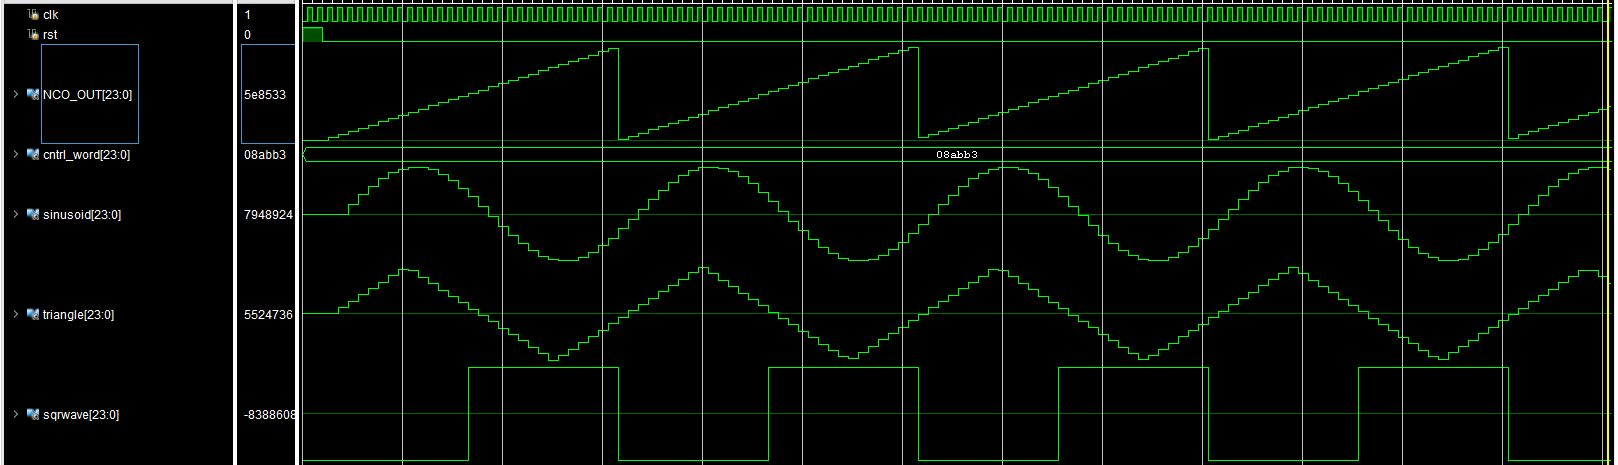
\includegraphics[scale=0.5]{simulation.JPG}	
	\end{center}
	\caption{DDS szimulációja}
	\label{a:simulation}
\end{figure}


\section{Éles teszt}

\begin{figure}[h!]
	\begin{center}
		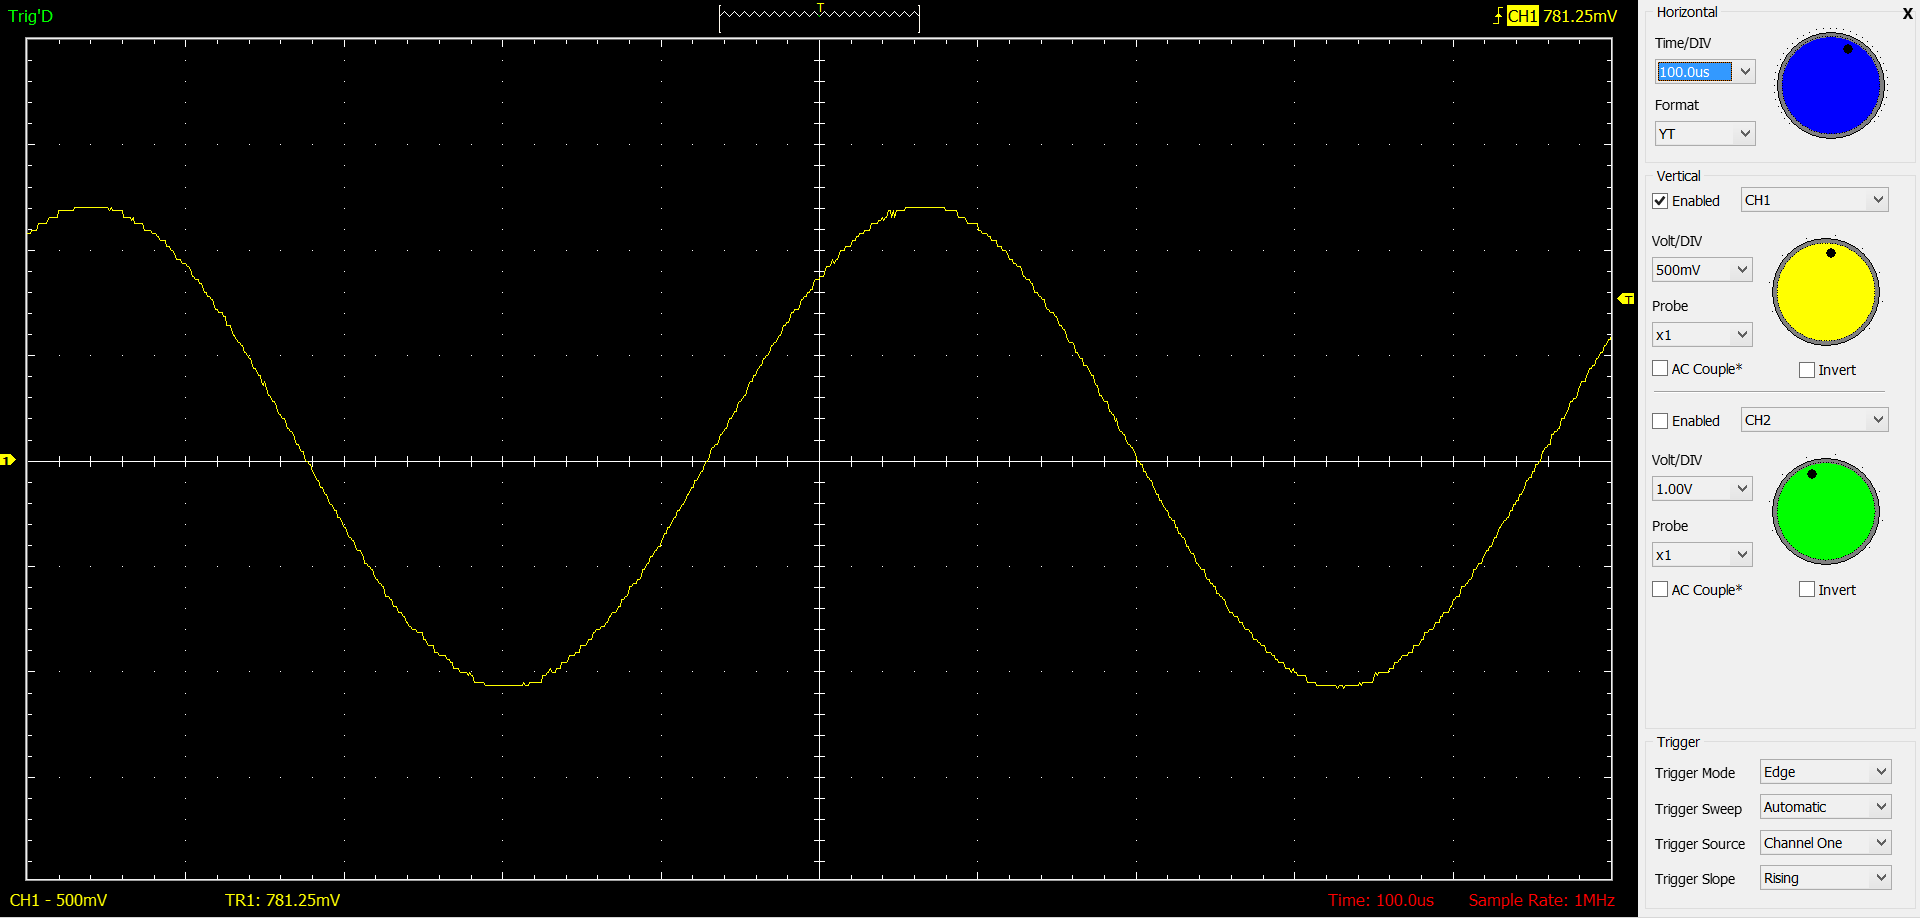
\includegraphics[scale=0.25]{scope_sin.png}	
	\end{center}
	\caption{Szinusz kimenet}
	\label{a:sinout}
\end{figure}

\begin{figure}[h!]
	\begin{center}
		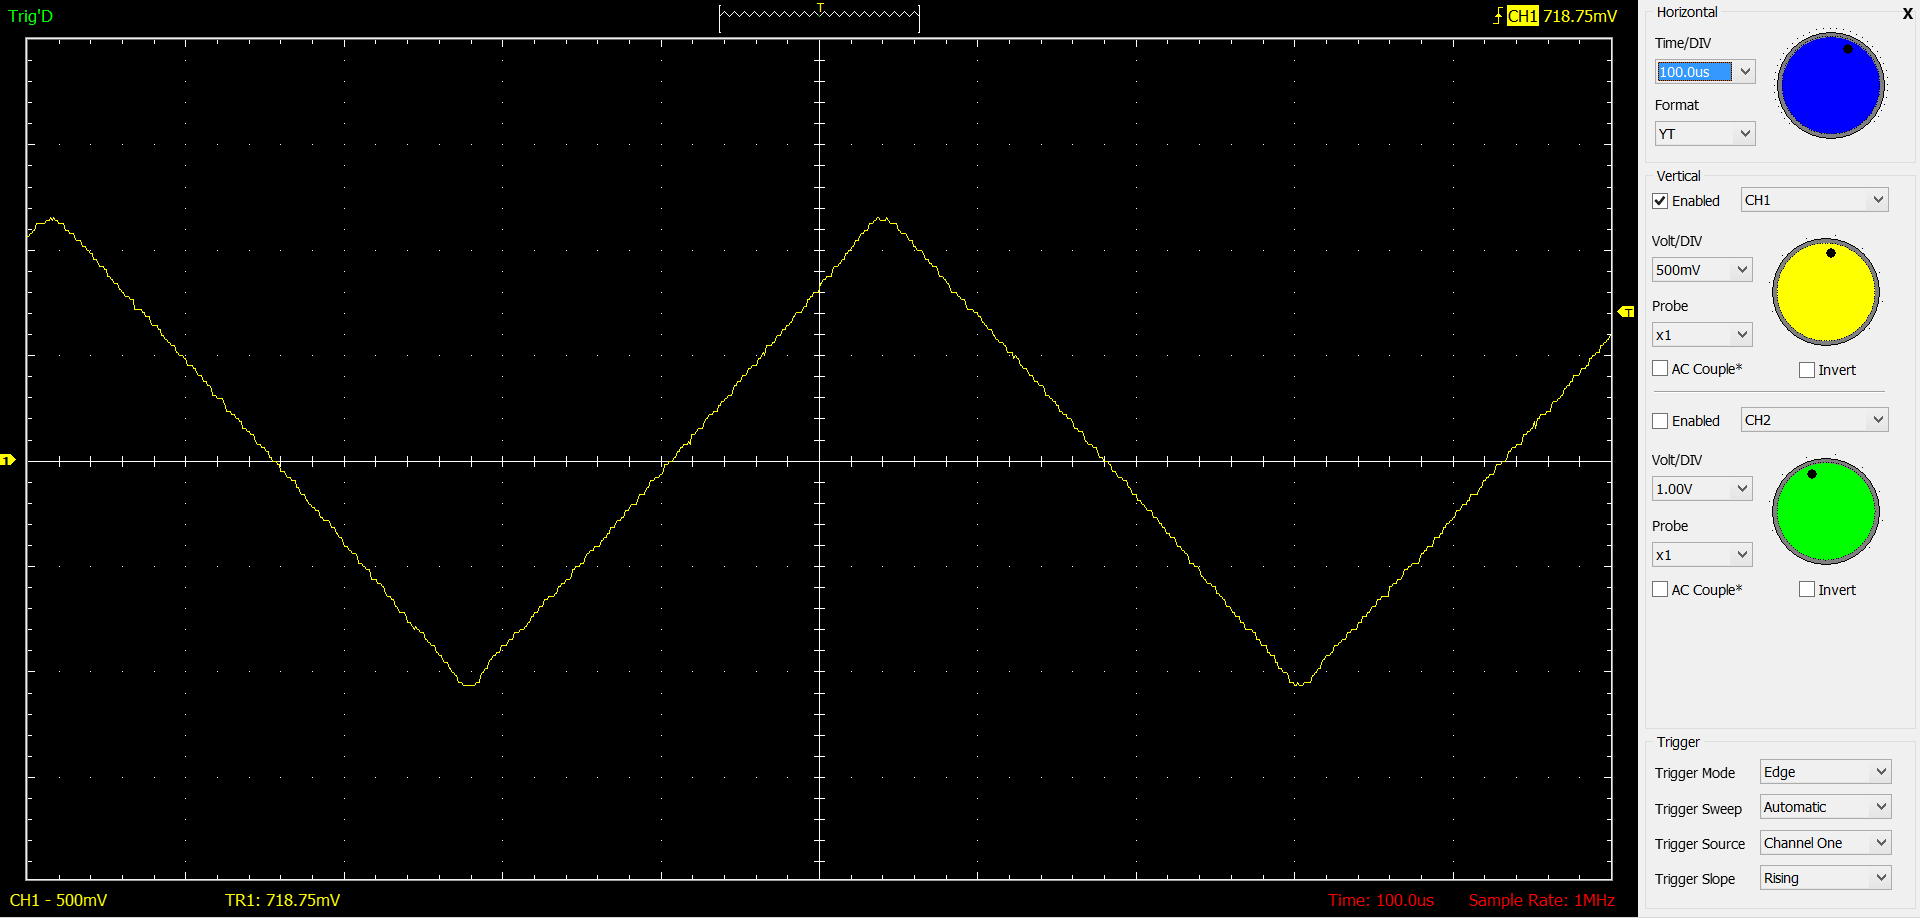
\includegraphics[scale=0.25]{scope_tri.png}	
	\end{center}
	\caption{Háromszögjel kimenet}
	\label{a:triout}
\end{figure}

\begin{figure}[h!]
	\begin{center}
		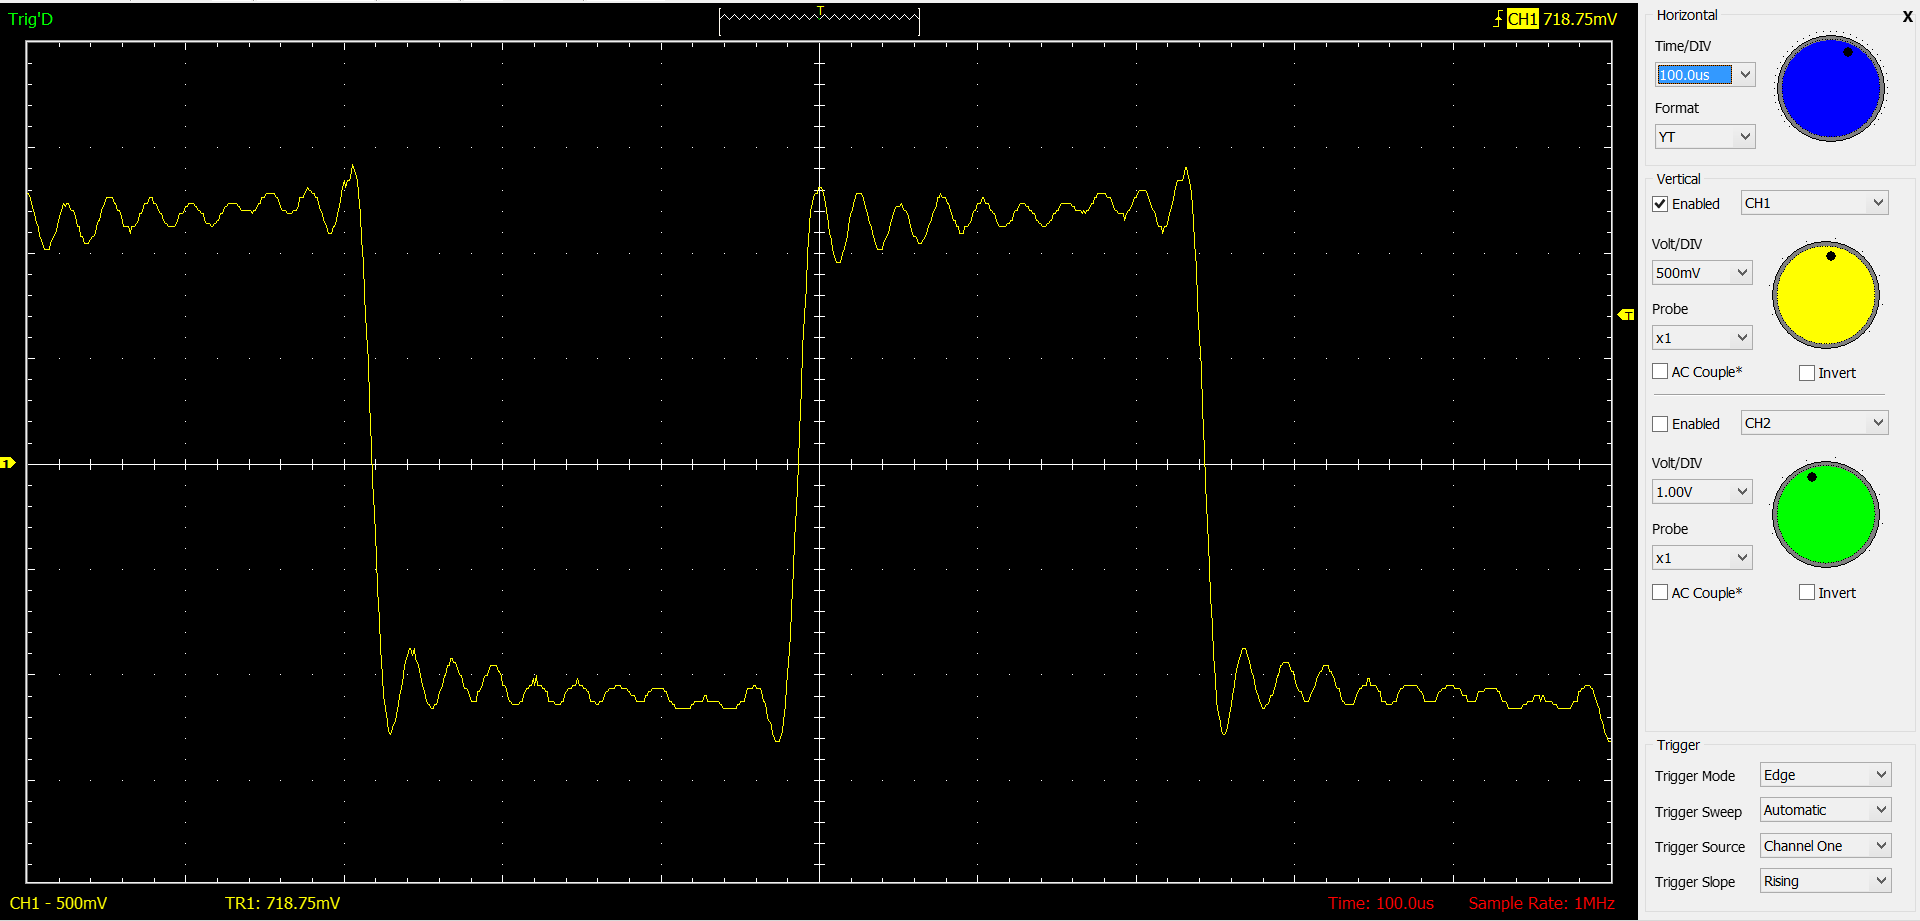
\includegraphics[scale=0.25]{scope_sqr.png}	
	\end{center}
	\caption{Négyszögjel kimenet}
	\label{a:sqrout}
\end{figure}

\section{Forráskód}

\subsection{DDS}

\lstinputlisting[
language=Verilog,
inputencoding=latin1,
basicstyle=\fontsize{7}{13}\selectfont\ttfamily,
keywordstyle=\color{blue}\ttfamily,
commentstyle=\color{OliveGreen}\ttfamily,
backgroundcolor = \color{lightgray}
]{../DDS/DDS.srcs/sources_1/new/DDS_top.v}

\subsection{Szinusz LUT}

\lstinputlisting[
language=Verilog,
inputencoding=latin1,
basicstyle=\fontsize{7}{13}\selectfont\ttfamily,
keywordstyle=\color{blue}\ttfamily,
commentstyle=\color{OliveGreen}\ttfamily,
backgroundcolor = \color{lightgray}
]{SIN_LUT.v}

\subsection{DDS toplevel}

\lstinputlisting[
language=Verilog,
inputencoding=latin1,
basicstyle=\fontsize{7}{13}\selectfont\ttfamily,
keywordstyle=\color{blue}\ttfamily,
commentstyle=\color{OliveGreen}\ttfamily,
backgroundcolor = \color{lightgray}
]{../DDS/DDS.srcs/sources_1/new/DDS_tl.v}


\pagebreak
\begin{thebibliography}{}

\bibitem{name1}

\textit{}
\url{  }
\today

\bibitem{name2}

\textit{Dither generátor}\\
\url{https://eewiki.net/pages/viewpage.action?pageId=16351401}

\today

\bibitem{name3}

\textit{}\\
\url{}
\today

\bibitem{name4}

\textit{}\\
\url{}
\today

\bibitem{name5}

\textit{}\\


\bibitem{name6}

\textit{}\\
\url{}
\today


\end{thebibliography}
\end{document}
